\section{Vypracování}

EM (Expectation-Maximization) algoritmus je jeden ze základních a velice efektivních přístupů, jenž je základem mnoha algoritmů strojového učení.
V konečném důsledku dochází k odhadu Gaussovských distribučních funkcí, které jsou generátory datové sady.

Samotný algoritmus se skládá ze 3 kroků:

\begin{enumerate}
    \item E-step;
    \item M-step;
    \item Výpočet chyby a návrat na bod 1.
\end{enumerate}

Před samotným výpočtem musíme stanovit prvotní odhad.
Podíváme-li se na rozložení dat (obrázek~\ref{fig:result1}), dokážeme odhadnout, že se v datech nachází 2 shluky.

\begin{figure}[htb]
    \centering
    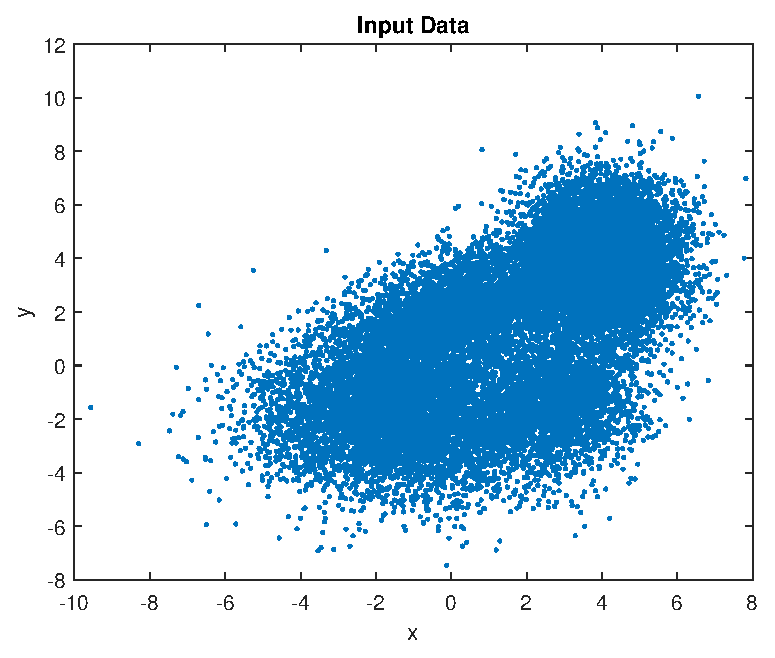
\includegraphics[width=0.55\textwidth]{graphs/fig1.eps}
    \caption{Vstupní data}
    \label{fig:result1}
\end{figure}
\FloatBarrier

Předpokládám symetričnost prvků Gaussovské směsi, tudíž \( \Sigma = I \).
Středy shluků \( \mu_1, \mu_2 \) byly určeny algoritmem \textit{k-means}, tudíž prvotní odhad je i řešením ke kterému bychom měli po několika iteracích dojít.
Počáteční váhy Normálních rozdělení byly zvoleny jako \( \frac{1}{\text{počet tříd}} = \frac{1}{2} \).

Výpočet byl proveden dvěma způsoby.
První výpočet je kontrolní, pouze s využitím funkcionalit softwaru MATLAB.
Výsledek tohoto výpočtu je na obrázku~\ref{fig:result2}.

\begin{figure}[htb]
    \centering
    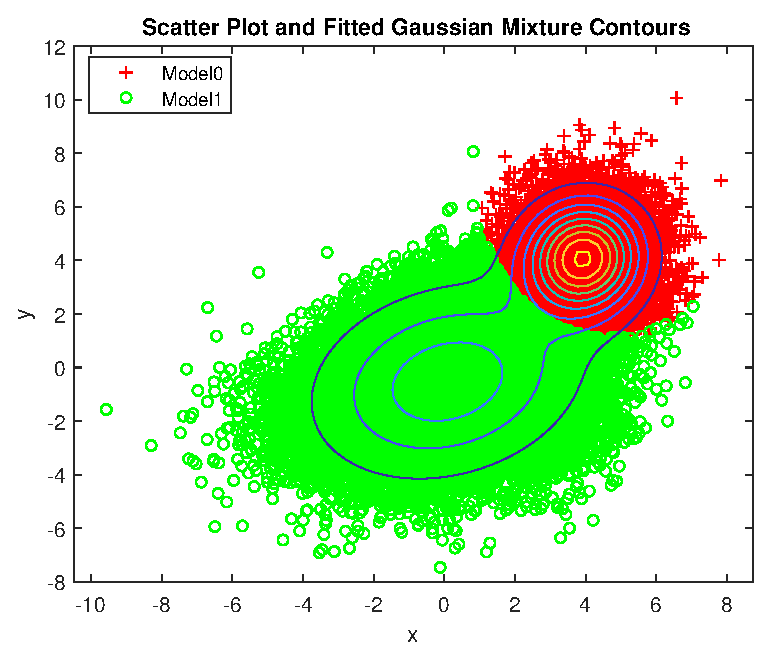
\includegraphics[width=0.55\textwidth]{graphs/fig2.eps}
    \caption{Výsledné rozdělení dat dle nativního EM algorimu}
    \label{fig:result2}
\end{figure}
\FloatBarrier

Graf~\ref{fig:result3} zobrazuje výsledek po výpočtu implementovaným E-M algoritmem.

\begin{figure}[htb]
    \centering
    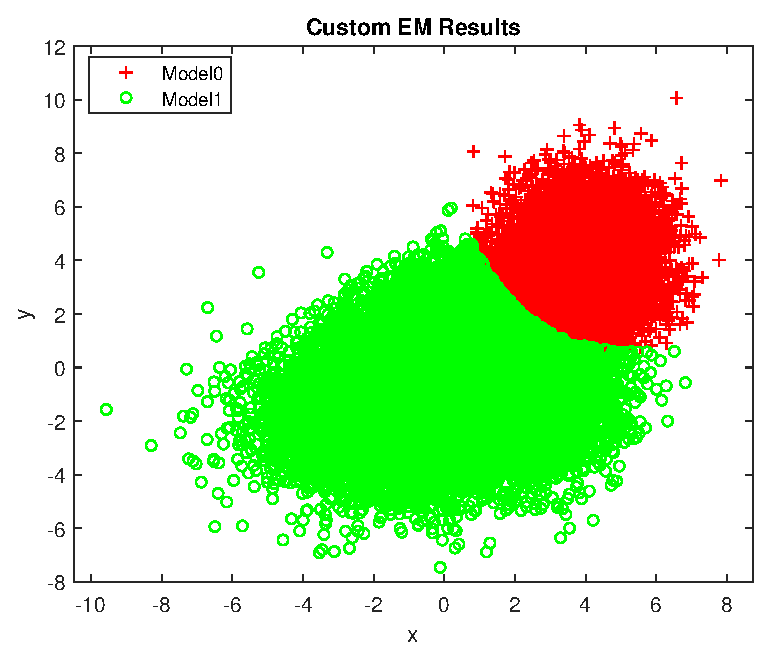
\includegraphics[width=0.55\textwidth]{graphs/fig3.eps}
    \caption{Výsledné rozdělení dat dle implementovaného E-M algorimu}
    \label{fig:result3}
\end{figure}
\FloatBarrier

Tabelované hodnoty dle zadání jsou v tabulce~\ref{table:table1}.

\begin{table}[htb]
    \centering

    \begin{tabular}{lrcccc}
        \toprule

        Iterace & Chyba     & \( \mu_1 \)       & \( \mu_2 \)       & \( \lambda_1 \)   & \( \lambda_2 \)   \\ \midrule
        1       & 0.0285    & [-0.4510 -1.2142] & [3.5411 3.6698]   & 0.5060            & 0.4940            \\
        2       & 0.1449    & [-0.3409 -1.1012] & [3.6216 3.7909]   & 0.4830            & 0.5170            \\
        3       & 0.1055    & [-0.2684 -0.9977] & [3.7013 3.8736]   & 0.4663            & 0.5337            \\
        4       & 0.0748    & [-0.2227 -0.9211] & [3.7617 3.9233]   & 0.4546            & 0.5454            \\
        5       & 0.0553    & [-0.1919 -0.8618] & [3.8086 3.9536]   & 0.4460            & 0.5540            \\
        6       & 0.0413    & [-0.1675 -0.8166] & [3.8453 3.9777]   & 0.4396            & 0.5604            \\
        7       & 0.0285    & [-0.1499 -0.7863] & [3.8689 3.9941]   & 0.4351            & 0.5649            \\
        8       & 0.0174    & [-0.1373 -0.7663] & [3.8831 4.0043]   & 0.4324            & 0.5676            \\
        9       & 0.0112    & [-0.1304 -0.7548] & [3.8921 4.0107]   & 0.4306            & 0.5694            \\
        10      & 0.0032    & [-0.1274 -0.7487] & [3.8970 4.0131]   & 0.4301            & 0.5698            \\
        11      & 0.0016    & [-0.1262 -0.7470] & [3.8982 4.0143]   & 0.4299            & 0.5701            \\
        12      & 0.0013    & [-0.1253 -0.7459] & [3.8989 4.0149]   & 0.4297            & 0.5703            \\
        13      & 0.0000    & [-0.1252 -0.7455] & [3.8993 4.0150]   & 0.4297            & 0.5703            \\
          
        \bottomrule
    \end{tabular}

    \caption{Tabulované hodnoty parametrů pro každou iteraci}
    \label{table:table1}
\end{table}
\FloatBarrier

Závislost chyby na počtu iterací je v grafu~\ref{fig:result4}.
Prvotní \enquote{velmi} přesný odhad (tedy malá chyba) je způsobena tím, že první odhad je vypočtem algoritmem \textit{k-means}.
Po následné reevaluaci rozložení dat ve shlucích jsou středy přepočteny a jelikož se jedná o teprve druhý krok algoritmu, tak tím hohužel znepřesněny.

\begin{figure}[htb]
    \centering
    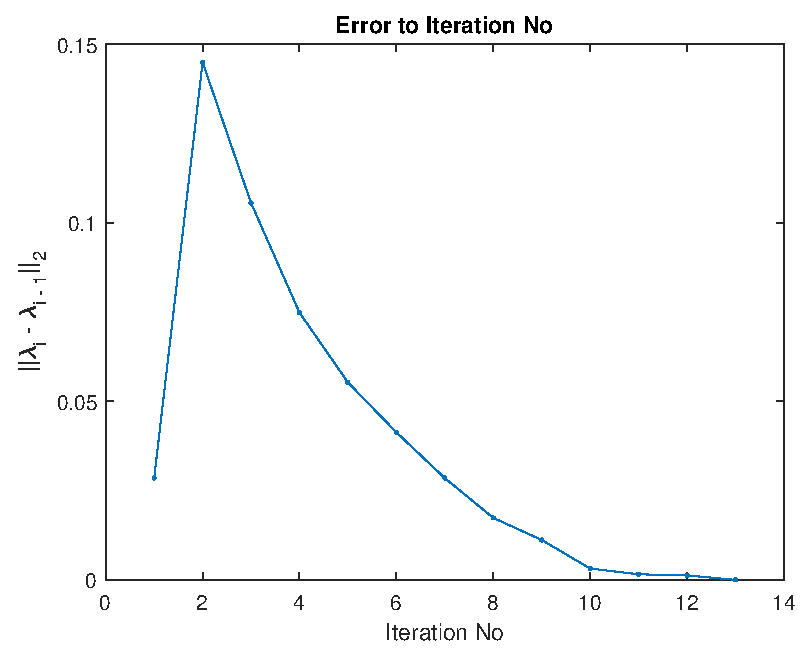
\includegraphics[width=0.55\textwidth]{graphs/fig4.eps}
    \caption{Hodnota chyby v každém uplynulém iteračním kroce}
    \label{fig:result4}
\end{figure}
\FloatBarrier

\section{Závěr}

Při řešení práce byly použity dvě varianty výpočtu.
Jelikož se tyto varianty shodují, lze přepokládat, že dostáváme správné výsledky.
Algoritmus dokovergoval ve 13. iteraci splněním zastavovací podmínky.
